\documentclass[12pt, a4paper]{article}
\usepackage[left=25mm, right=25mm, top=25mm, bottom=25mm]{geometry}
\usepackage{graphicx}
\usepackage{amsmath}
\usepackage{natbib}
\usepackage{comment}
\usepackage{caption}
\usepackage{subcaption}
\usepackage{tikz}
\usepackage{setspace}
\usepackage{xfrac}
\usepackage{rotating}
\usepackage{float}
\usepackage{mathptmx}
\usepackage{xurl}
\usepackage[section]{placeins}
\usepackage{color}   % to colour links
\usepackage{hyperref}
\usepackage{caption}
\usepackage[super]{nth}
\usepackage{cleveref}
\usepackage{listings}

%%%%%%%%%%%%%%%%%%%%%%%%%%%%%%%%%%%%%%%%%%%%%%%%%%%%%%%%%%%%%%%%%%%%%%%

\usetikzlibrary{positioning}
%\bibliographystyle{plain}
\bibliographystyle{unsrt}
\graphicspath{{./images/}}

\definecolor{codegreen}{rgb}{0,0.6,0}
\definecolor{codegray}{rgb}{0.5,0.5,0.5}
\definecolor{codepurple}{rgb}{0.58,0,0.82}
\definecolor{backcolour}{rgb}{0.95,0.95,0.92}

\PassOptionsToPackage{hyphens}{url}\usepackage{hyperref}
\hypersetup{
    colorlinks=true,  % set true if you want colored links
    linktoc=all,      % set to all if you want both sections and subsections linked
    linkcolor=black,  % choose some color if you want links to stand out
    citecolor=black,
    urlcolor=blue
}

\setlength{\parindent}{5ex}
\onehalfspacing

\title{Mechanics Walk Sections}
\author{Aidan Lee}
\date{July 2021}

\begin{document}

\maketitle
\section{Motivation}

The early exposure of younger elementary-aged students to STEM topics has a positive impact in cultivating interest and aspiration. By capturing this demographic's interest at an early stage, more students to undergo the groundwork in secondary school to enter STEM fields \cite{dejarnette_americas_2012}.

Science museums have been particularly successful in bridging the gap between scientists and laymen, with interactable models that are entertaining and facilitate 'accidental' learning \cite{tressel_role_1980}. These recreational learning exhibits generate interest in STEM for a wide audience. Physical and interactive demonstrations are excellent to do so. Teaching mechanics without an interactive physical model is similar to teaching someone seated at a desk how to ride a bike.

The aim of this project is to create an awareness of mechanics in a younger demographic by creating alluring and interesting interactive models that lead to recreational and ``accidental'' learning, that also provide the option for further learning.


\section{Progress and Methodology}
This project entails the creation of several physical interactable models that each demonstrate a mechanical concept or phenomenon. These models would be placed around the campus in University College Dublin with a graphic at each location to direct the attendee to the next location. This graphic will also provide brief instructions of how to interact with the model to observe the desired mechanical phenomenon, and will include a QR code that directs the attendee to a webpage, where the mechanics of the phenomenon will be explained.

In this way, the models can achieve the objective of being recreational activities that encourage "accidental learning". If the attendee is interested in learning the theory in a more traditional sense, they have the option through the QR code.

As the objective of this project was to attract younger children to mechanics, the demonstrations needed to be interesting. This project aims to achieve this by choosing models that demonstrate strange physics phenomena that exhibit unintuitive behaviour with a cause that is not immediately apparent. By being "unintuitive", each model should do the unexpected. This will make the demonstrations more engaging as it first confuses the viewer and makes them think about the reason behind the phenomena. However for this confusion to occur, the base mechanics of the phenomena need to be tangible enough for the initial intuition to be applied.

9 phenomena and demonstrations were chosen to be included in this project. These were the brachistochrone problem, Galton board, double pendulum, coupled oscillators, nails-in-a-box, gyroscopic precession, metronome synchronisation, tensegrity structure, and an uphill roller. Combined, these demonstrate the central limit theorem, the butterfly effect, how order can form due to minimum energy states, precession, spontaneous synchronisation, Newton's 1st law and centres of gravity.

\begin{figure}[H]
    \centering
    \begin{subfigure}{.5\textwidth}
        \centering
        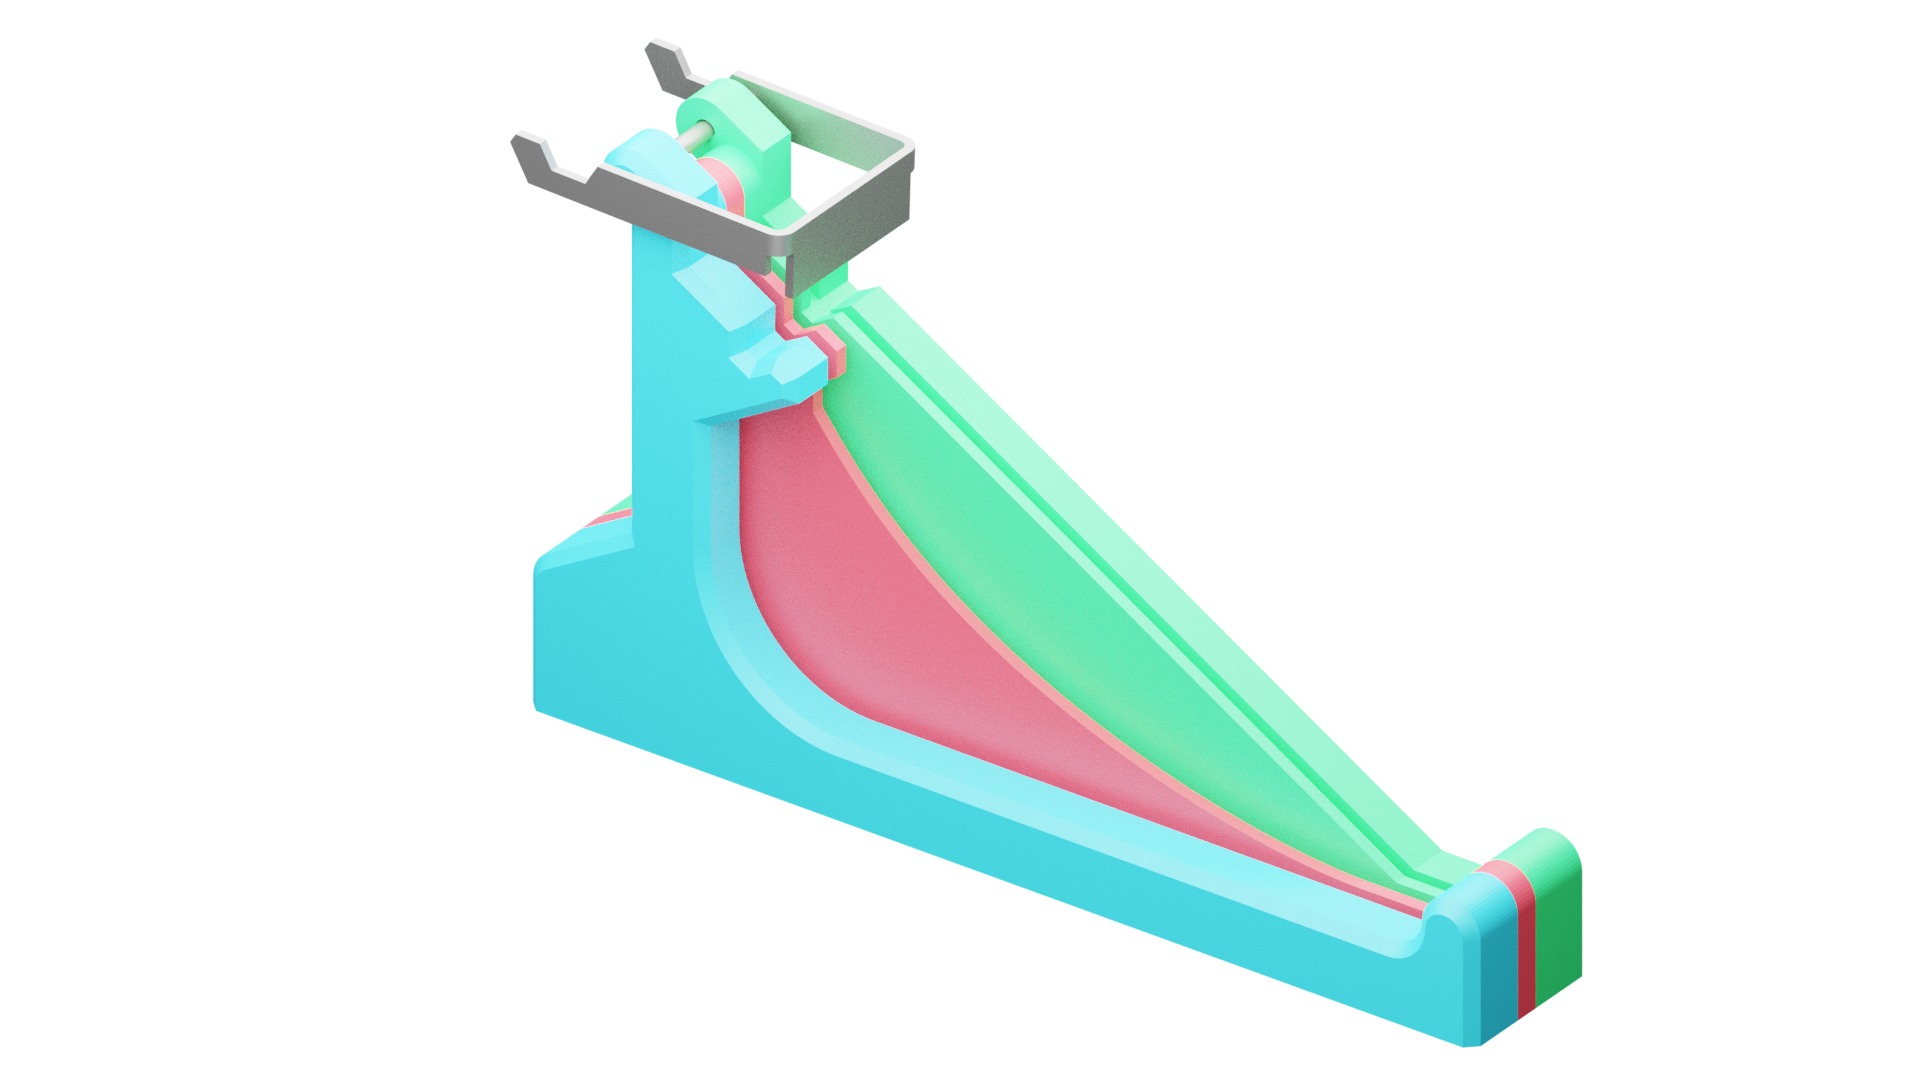
\includegraphics[width=8cm]{BR-render-1.png}
        \caption{Curved paths}
        \label{}
    \end{subfigure}%
    \begin{subfigure}{.5\textwidth}
        \centering
        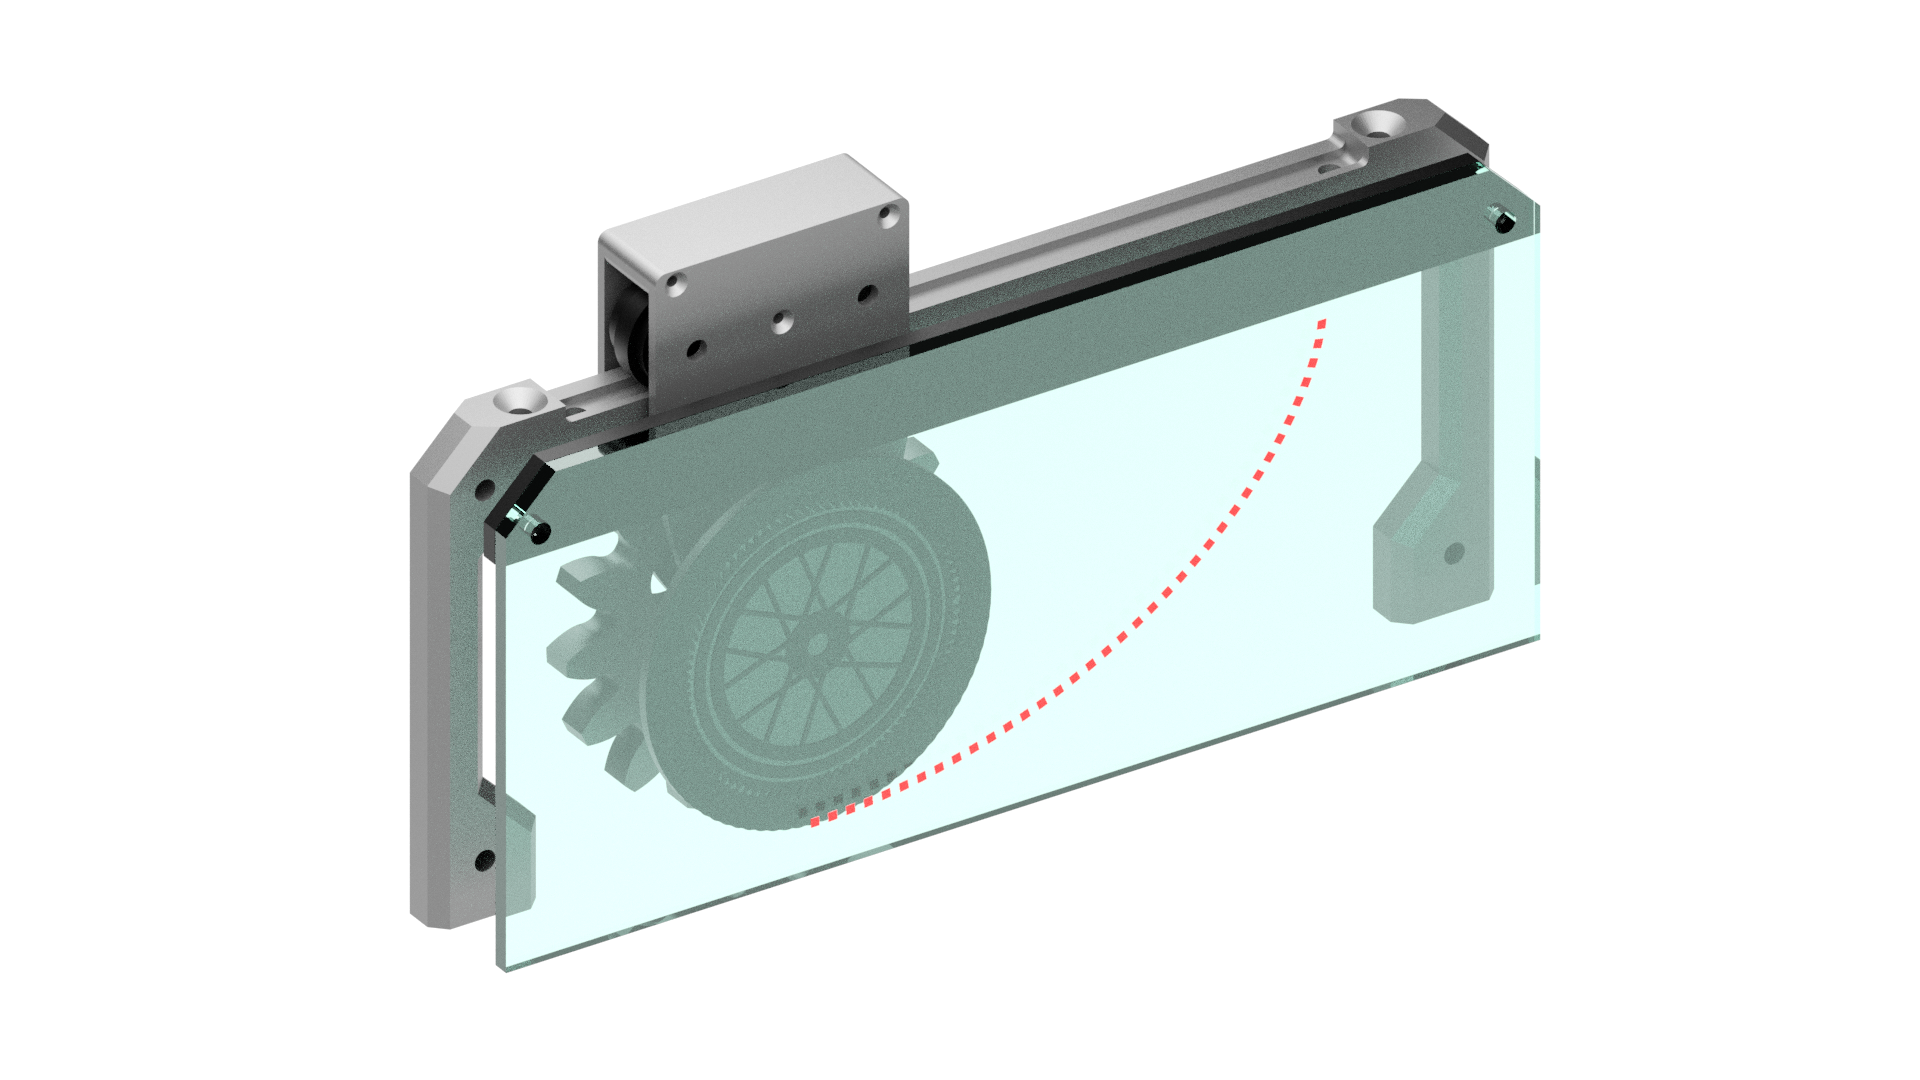
\includegraphics[width=8cm]{BR-render-2.png}
        \caption{Cycloid drawer}
        \label{}
    \end{subfigure}
    \caption{Brachistochrone model}
    \label{brachistochrone}
\end{figure}
In the Brachistochrone model, one might expect the shortest path of the line to be the fastest point between the start and end positions. However, the fastest path is a curve that is the segment of a cycloid. The model includes a rack and pinion that is turned such that a cycloid is graphed.

\begin{figure}[H]
    \centering
    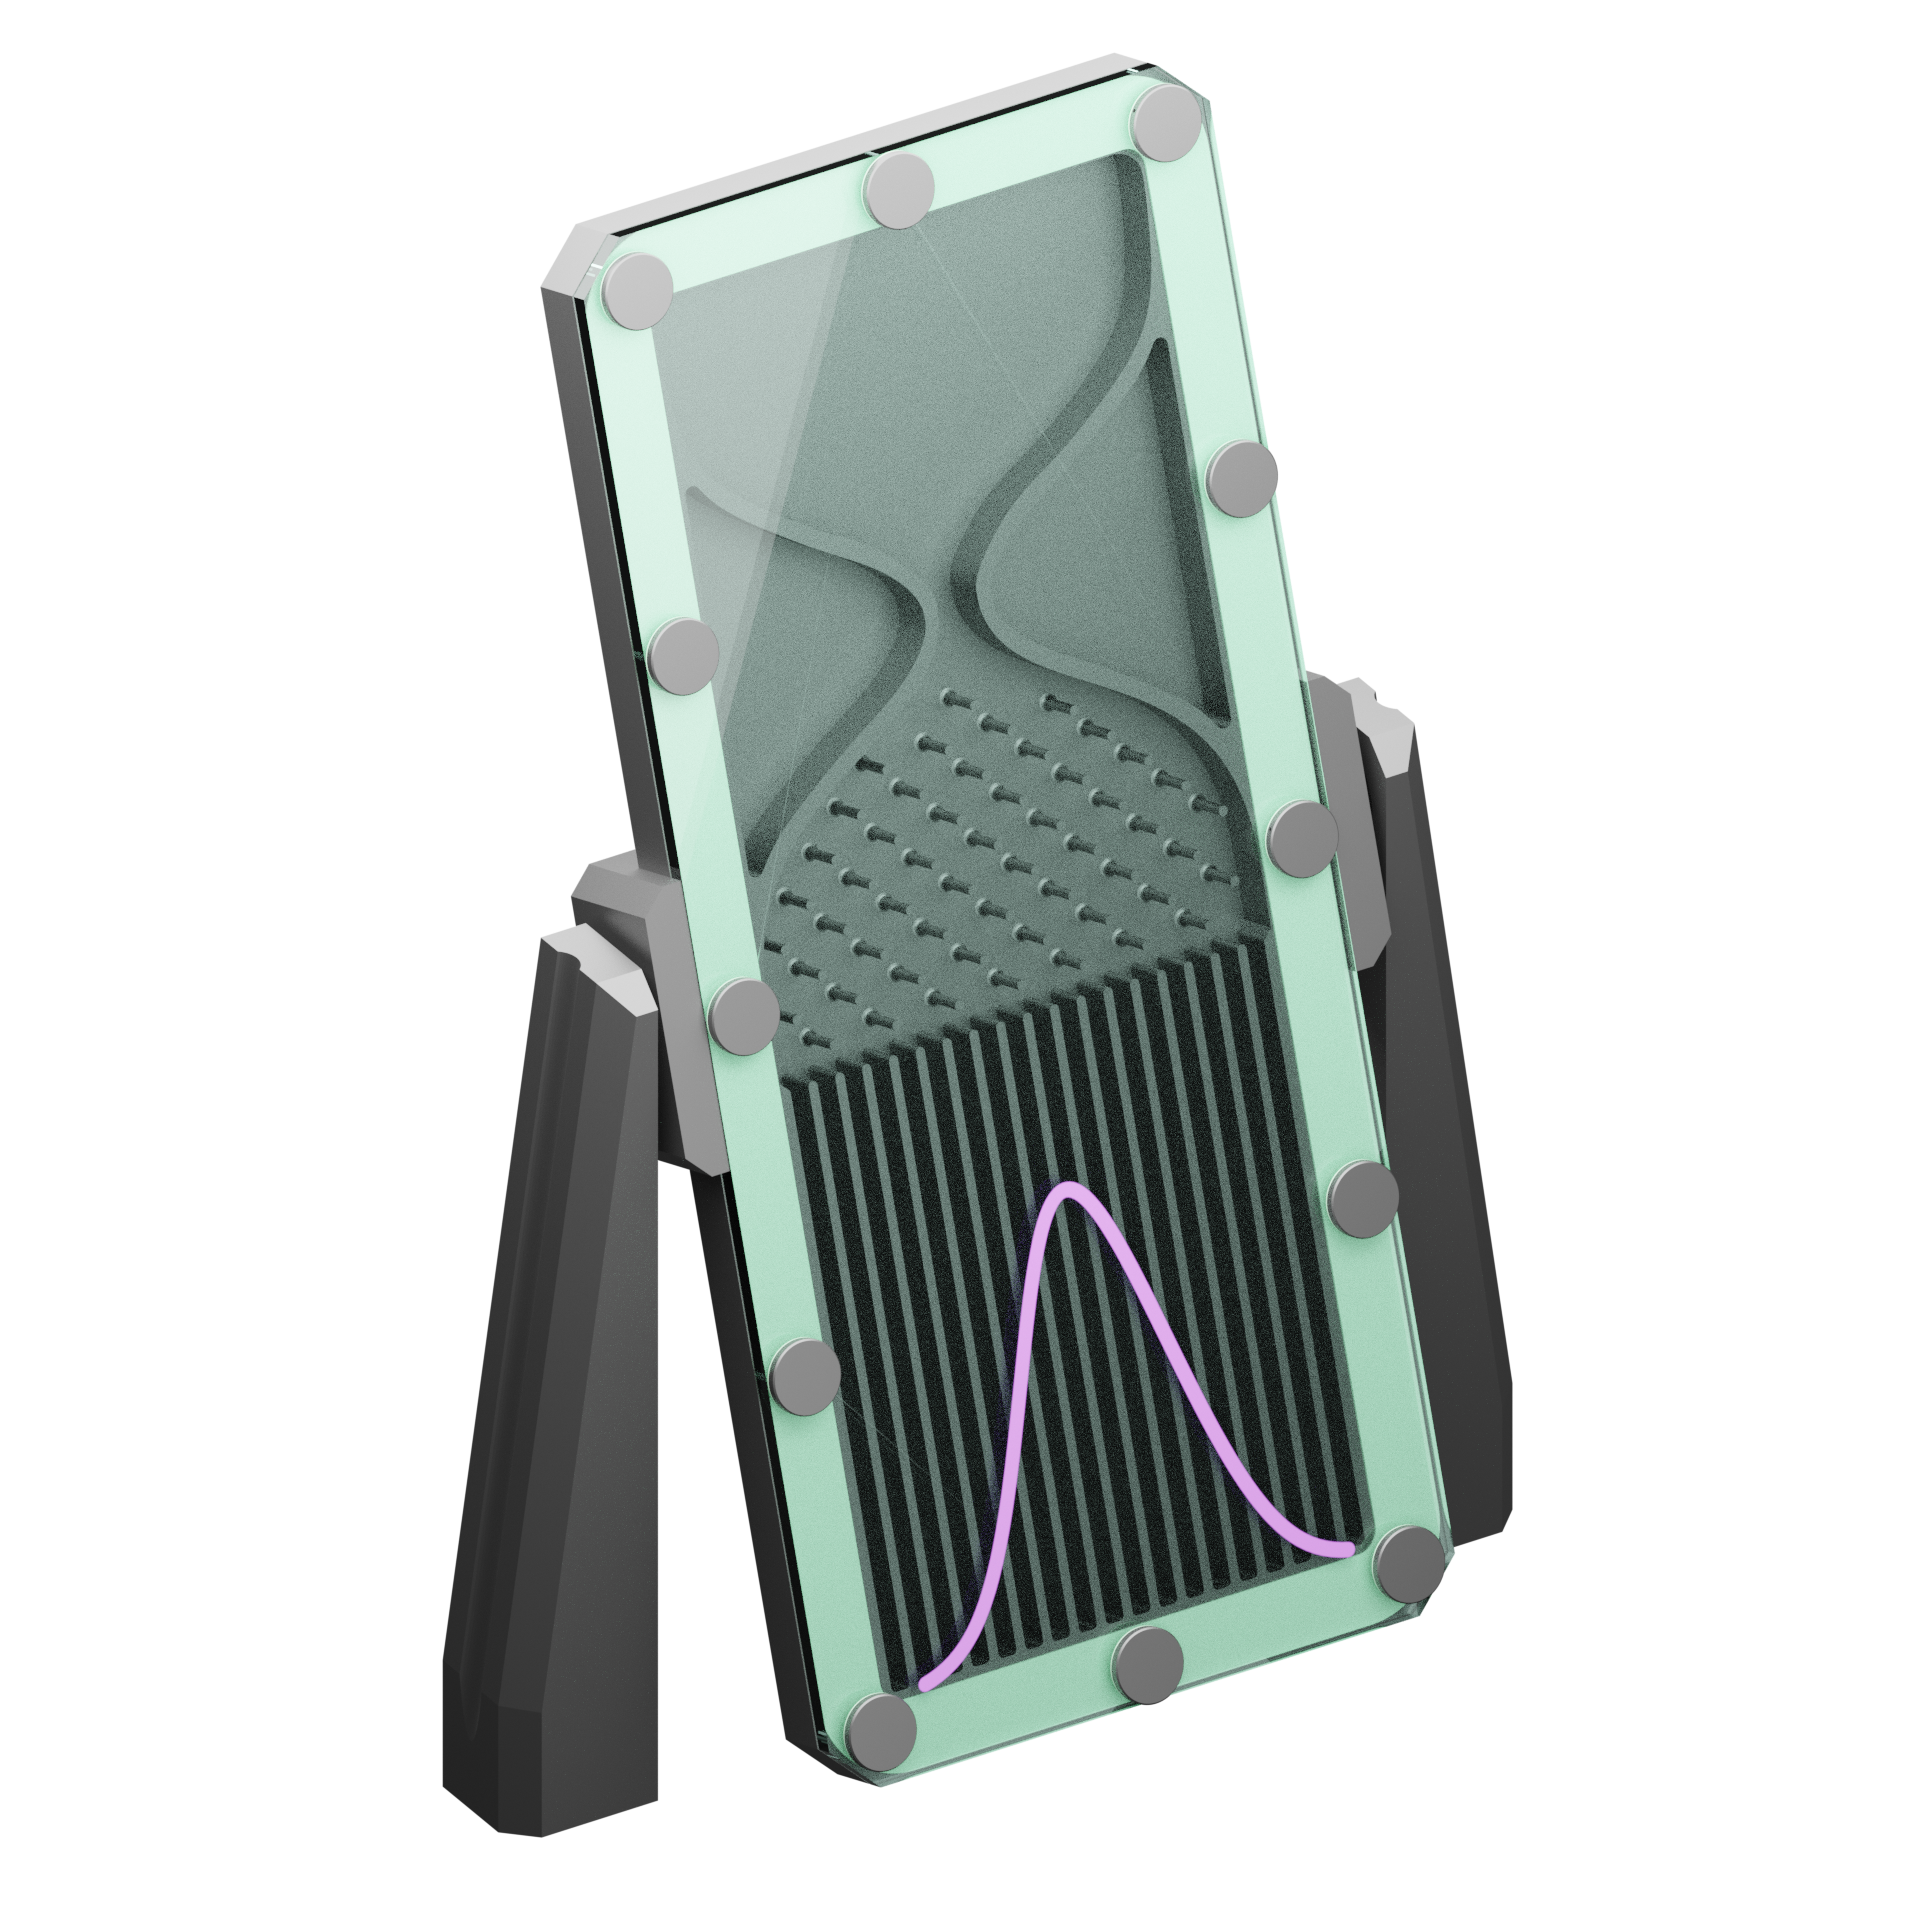
\includegraphics[width=8cm]{GaltonBoard-render-sticker.png}
    \caption{Galton board}
    \label{galtonboard}
\end{figure}
The Galton board demonstrates the central limit theorem. In this model, a series of balls fall under gravity, into an array of pegs. After hitting a peg, each ball has a 50/50 chance of going to the left or right peg below it. After many balls have gone through this array of pegs, the result at the bottom is a normal distribution. 
One may not expect such a stochastic system to produce the same result in every run of the experiment. However, as the attendee repeats the experiment by flipping the board, they will find that the resulting distribution at the bottom is the same every time, despite the final location of an individual ball being unpredictable. 
% not good enough

\begin{figure}[H]
    \centering
    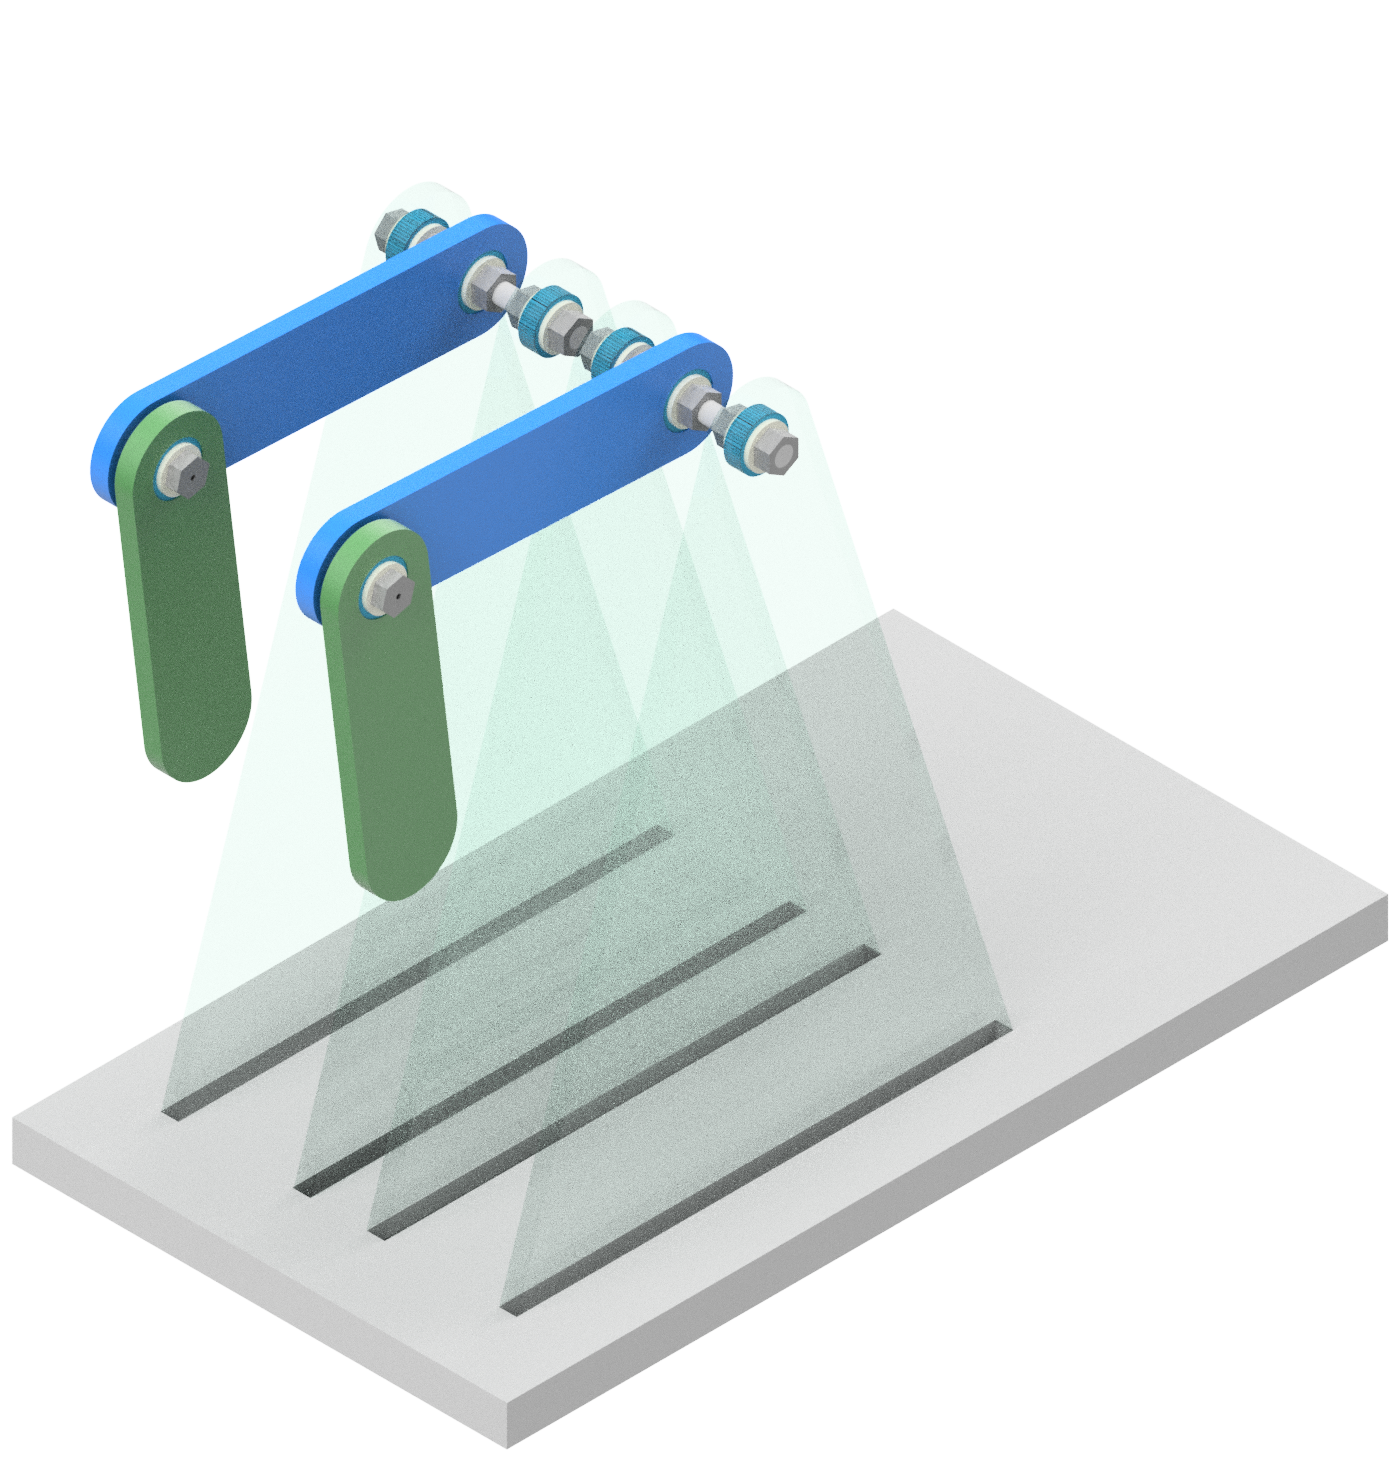
\includegraphics[width=8cm]{DBP-assembly-render.png}
    \caption{Double pendulum}
    \label{}
\end{figure}
The double pendulum demonstrates chaos and the butterfly effect, which refers to the extreme sensitivity of an outcome to the initial conditions that occurs in chaotic systems. This demonstration has the attendee start 2 double pendulums the same way, such that the pendulums are expected to follow the same path. However, the user will observe that the 2 pendulums will take completely different trajectories after some time due to the butterfly effect.

\begin{figure}[H]
    \centering
    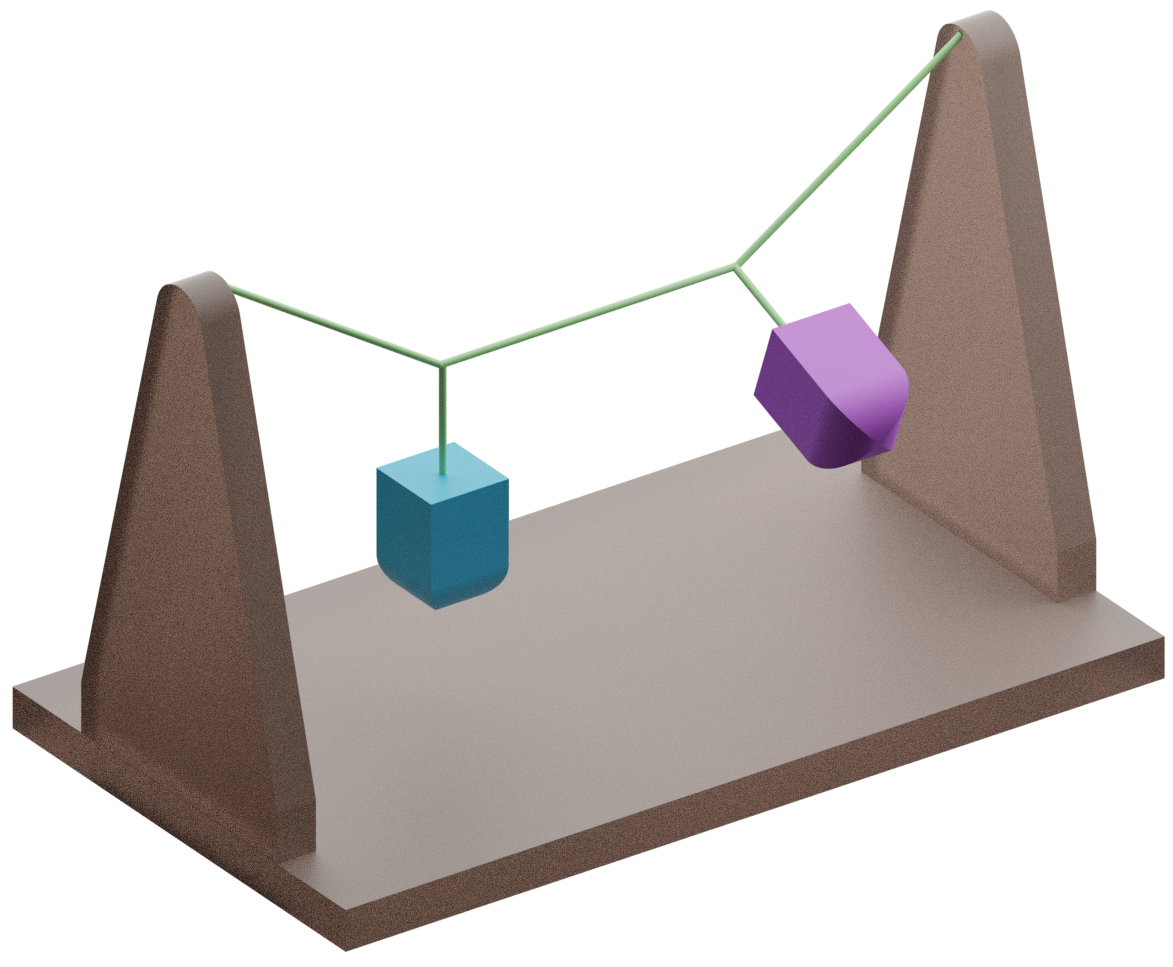
\includegraphics[width=8cm]{CPO-assembly.png}
    \caption{Coupled oscillators}
    \label{}
\end{figure}
The coupled oscillators model has 2 pendulums connected to a loose string or rope. When the attendee starts one pendulum, they will see the pendulums couple and the energy transfer that leads to the 2 pendulums taking turn swinging.

The nails-in-a-box model is highly interactive as it has the attendee shake a box in a regular manner from side to side. Inside the box, there are initially mixed up nails, which order themselves as the attendee provides them with energy to rearrange in a highly organised manner. In this way, the model demonstrates minimum energy states and how order can arise from chaos. 
% is this true?

\begin{figure}[H]
    \centering
    \begin{subfigure}{.5\textwidth}
        \centering
        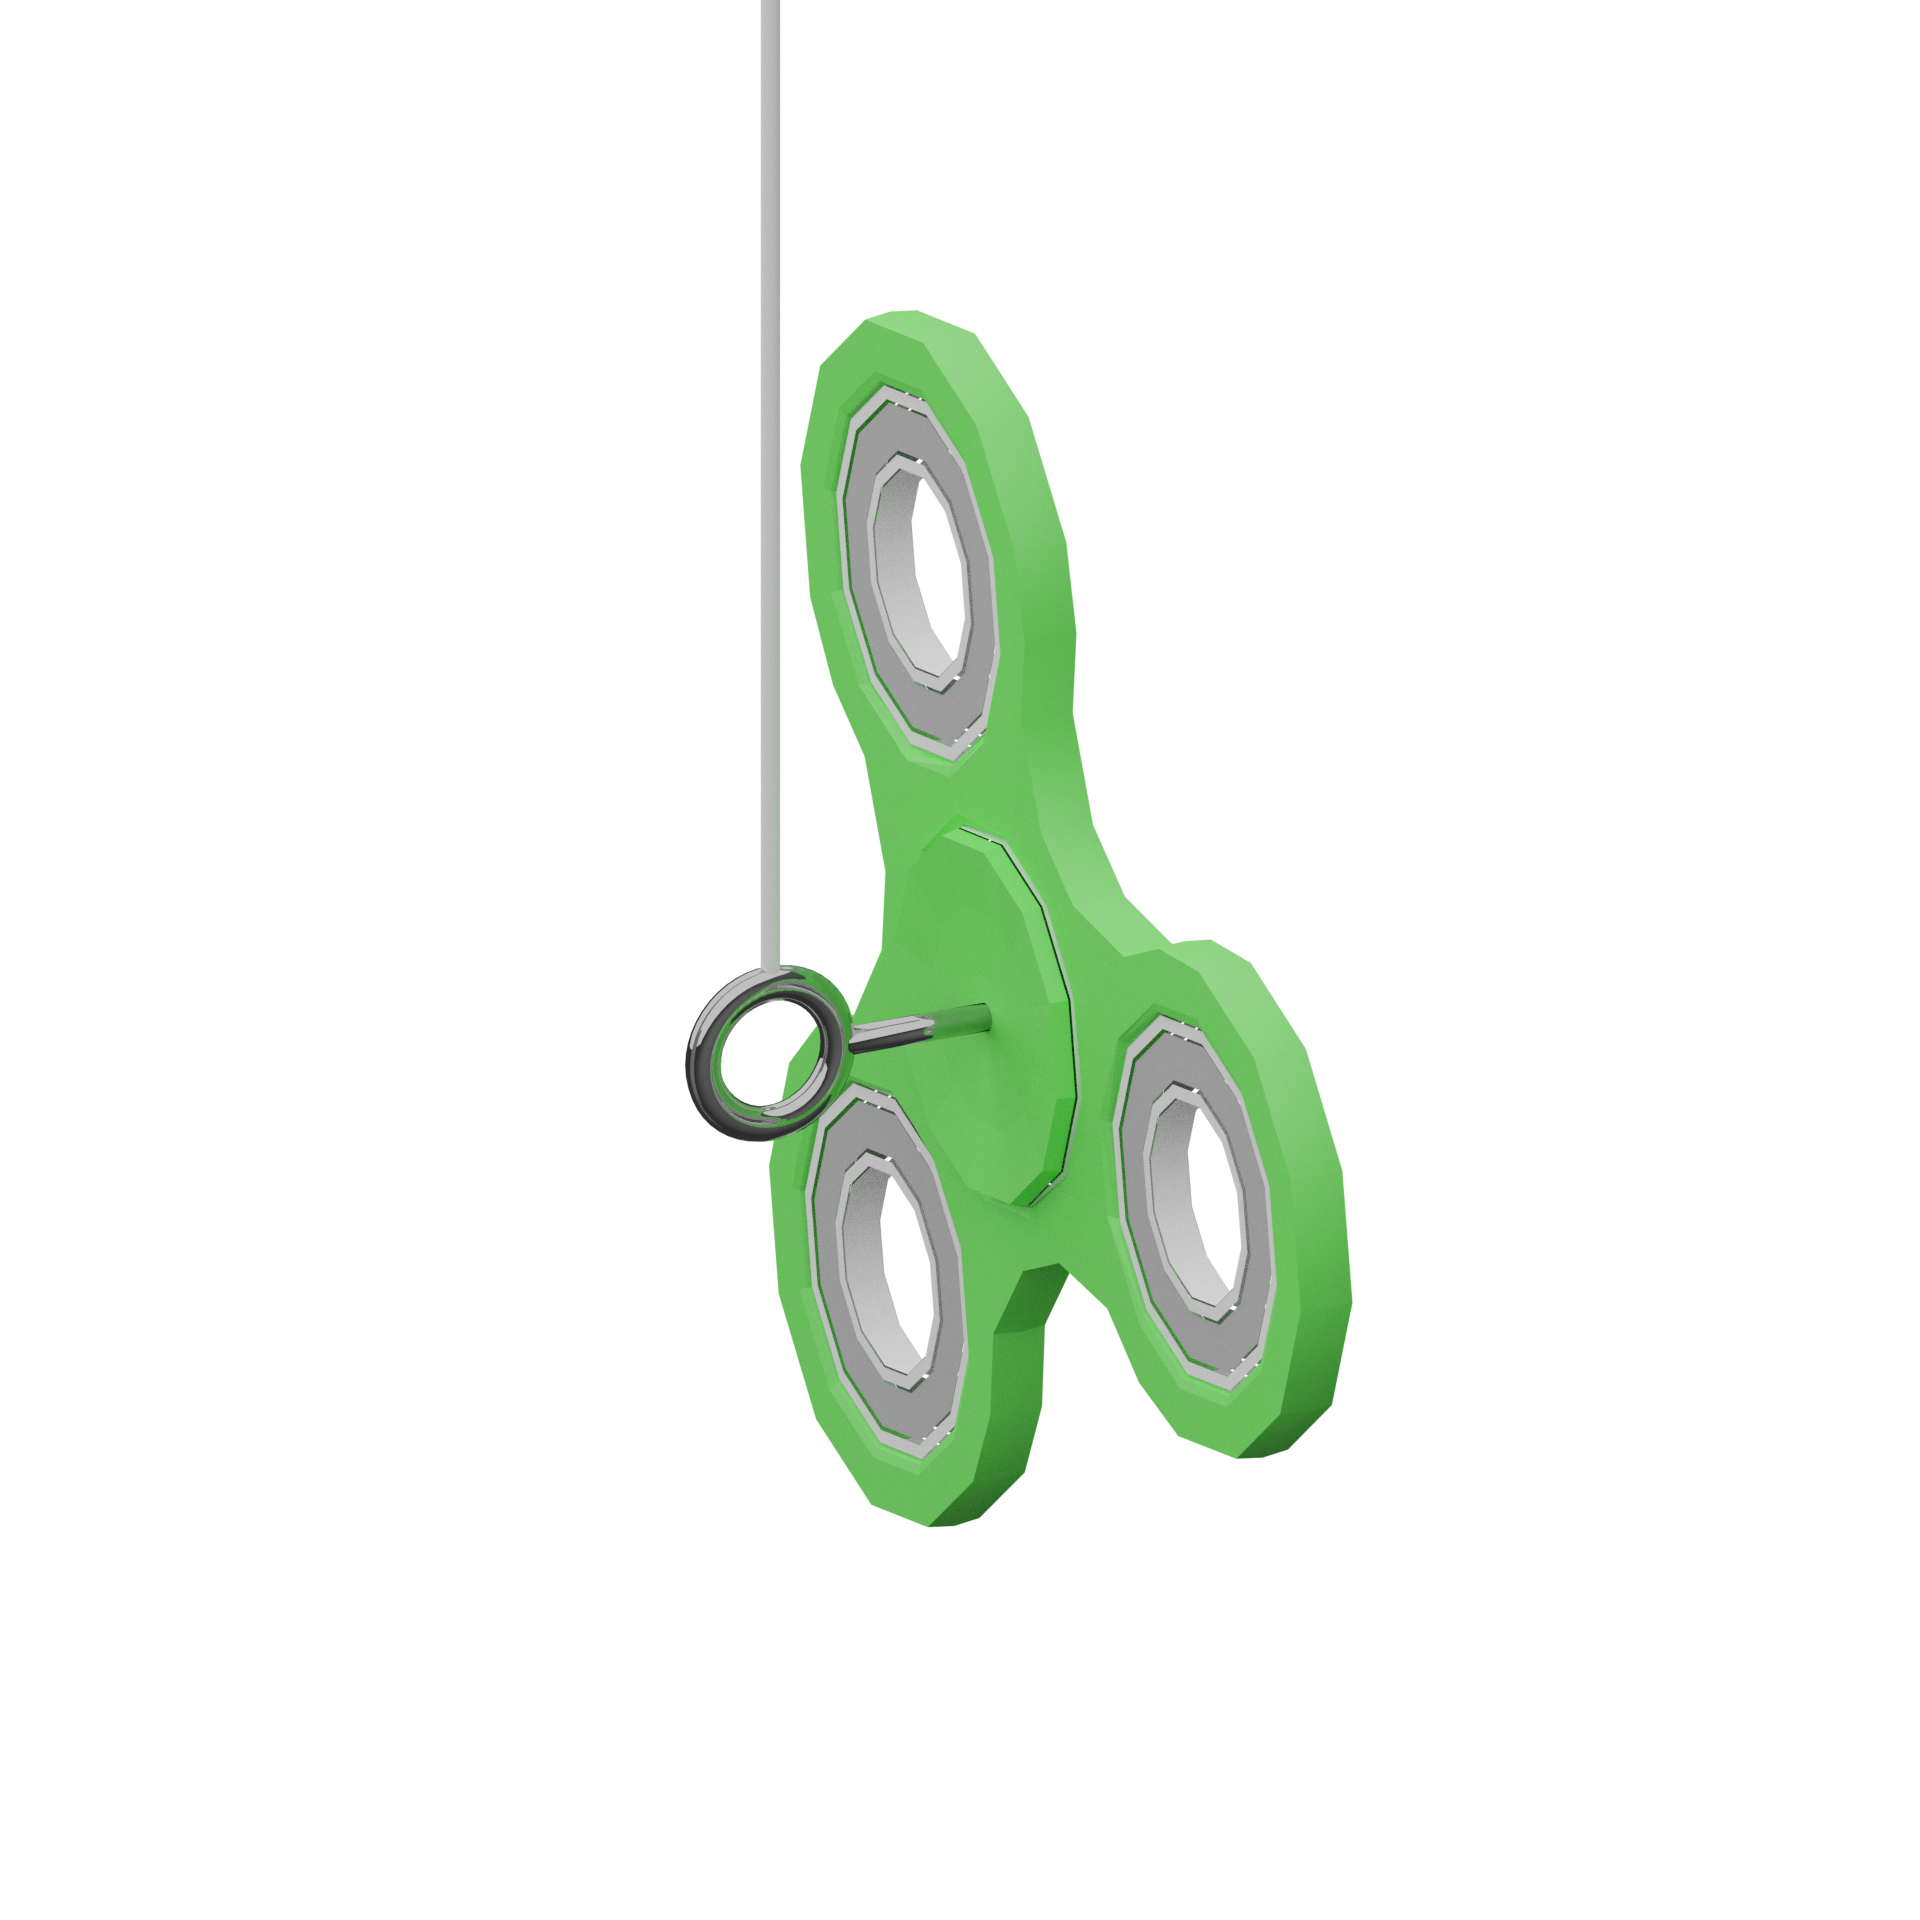
\includegraphics[width=8cm]{stoppedfidget.png}
        %\caption{}
        \label{}
    \end{subfigure}%
    \begin{subfigure}{.5\textwidth}
        \centering
        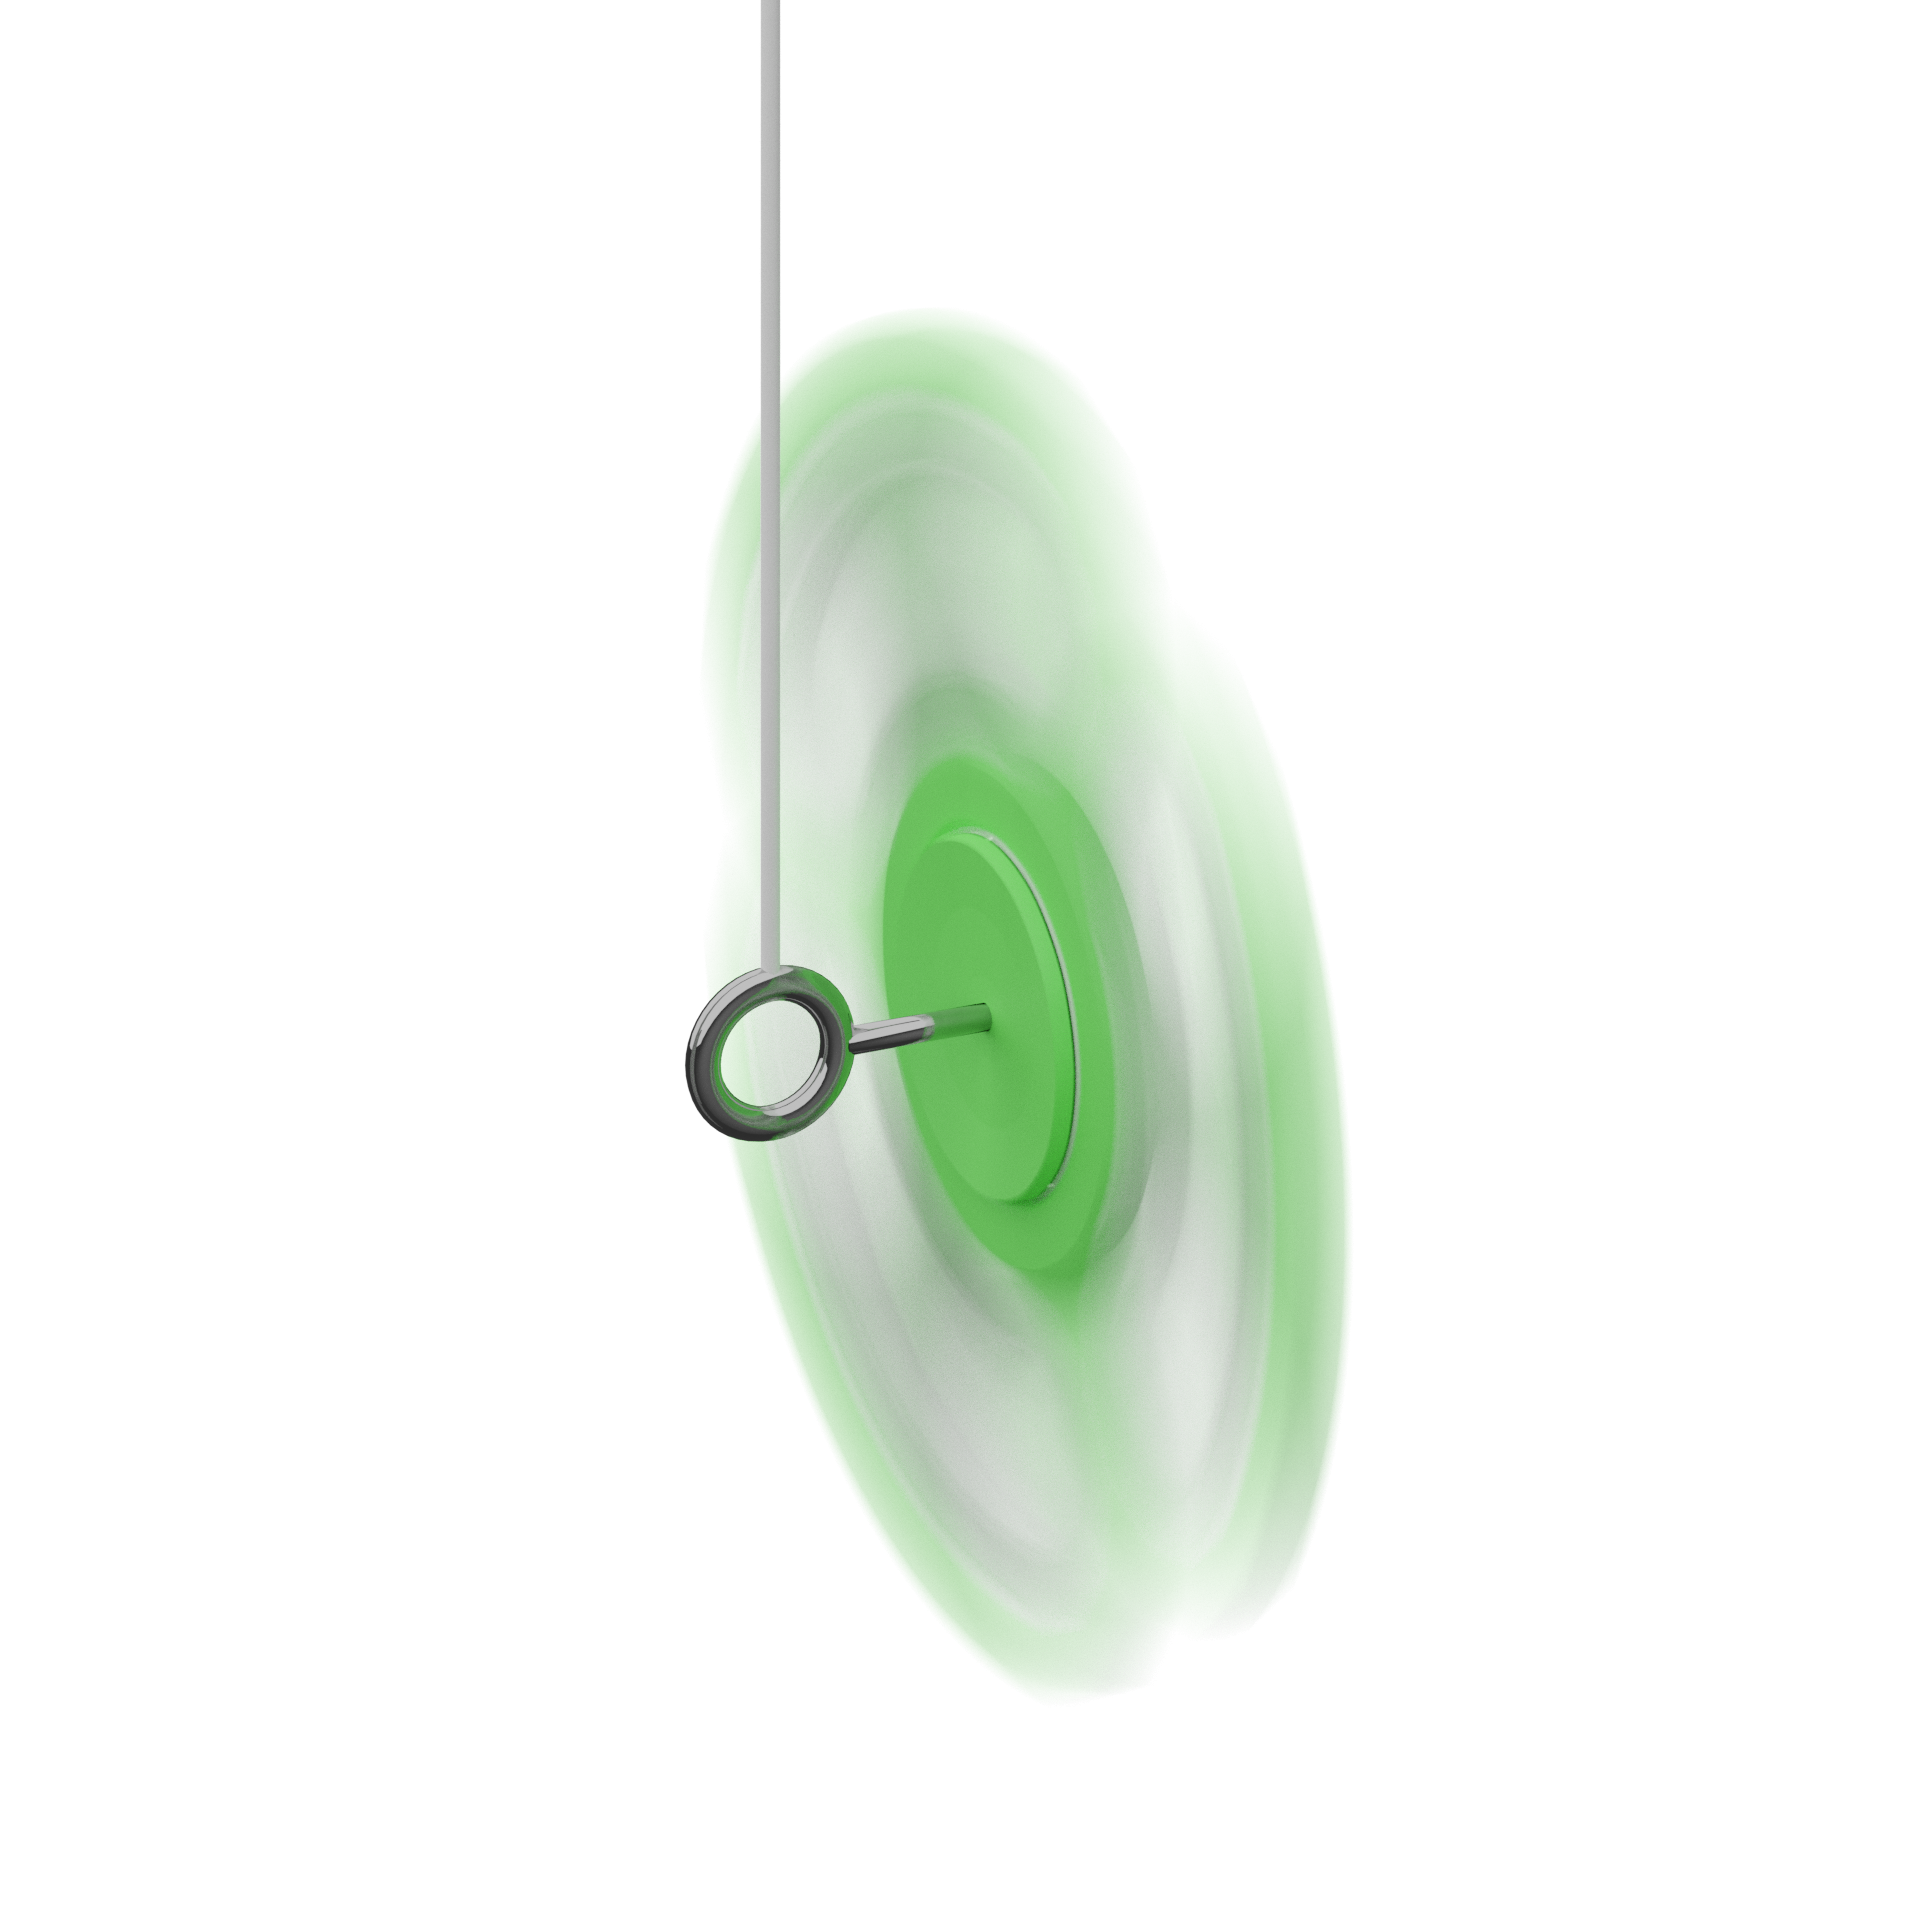
\includegraphics[width=8cm]{spinningfidget.png}
        %\caption{}
        \label{}
    \end{subfigure}
    \caption{Fidget Spinner Demonstrating Gyroscopic Precession}
    \label{precession}
\end{figure}
Gyroscopic precession is demonstrated by a fidget spinner at the end of a string. A small screw hook connects the spinner to the string as show in Fig~\ref{precession}. When the spinner is spun and released by the attendee, it gyroscopically precesses.


\begin{figure}[H]
    \centering
    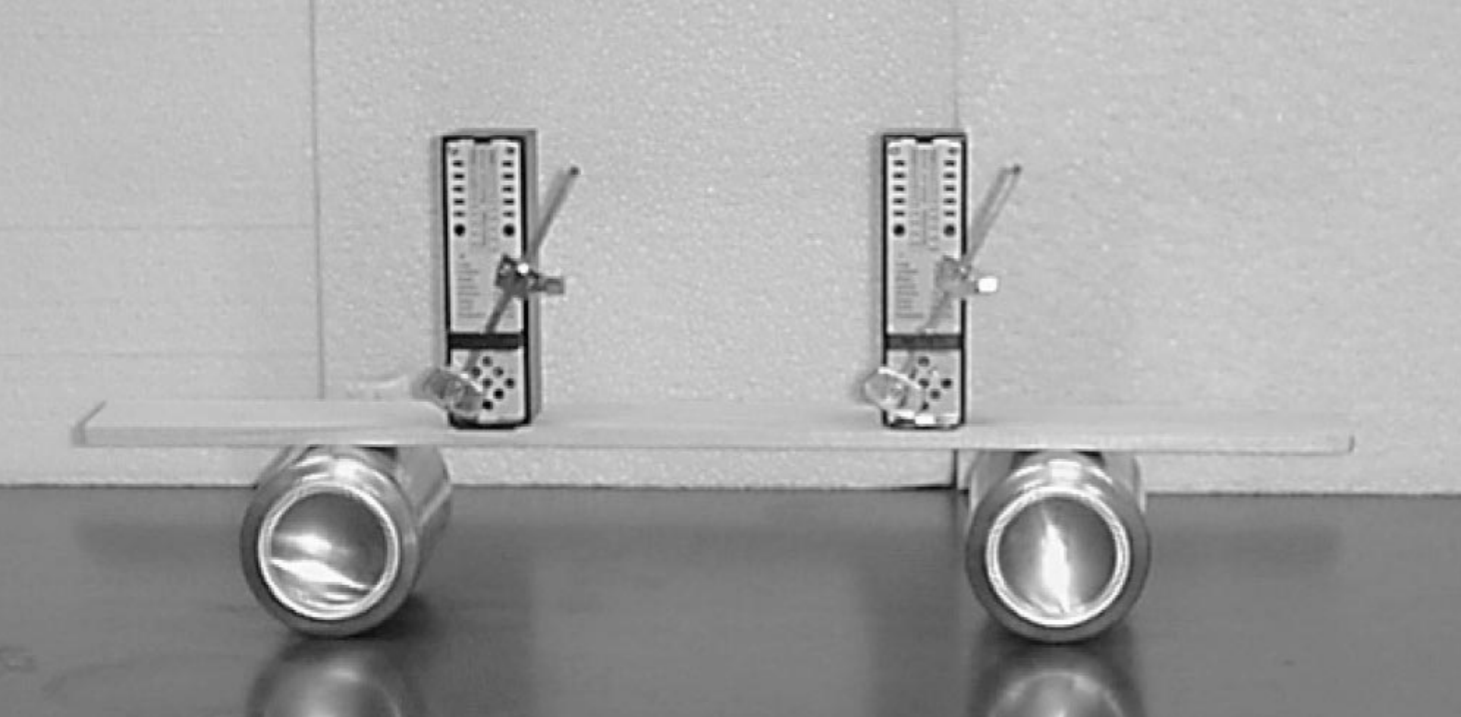
\includegraphics[width=8cm]{metronomes2.png}
    \caption{Spontaneous synchronisation of metronomes \cite{pantaleone_synchronization_2002}}
    \label{metronomes}
\end{figure}
Spontaneous synchronisation is exhibited by the classic demonstration of metronomes on a platform that is allowed to roll in the swing direction of the metronome bars. After the attendee starts the metronomes, they start to synchronise after some time.
% written for a reader that already knows mechanics

\begin{figure}[H]
    \centering
    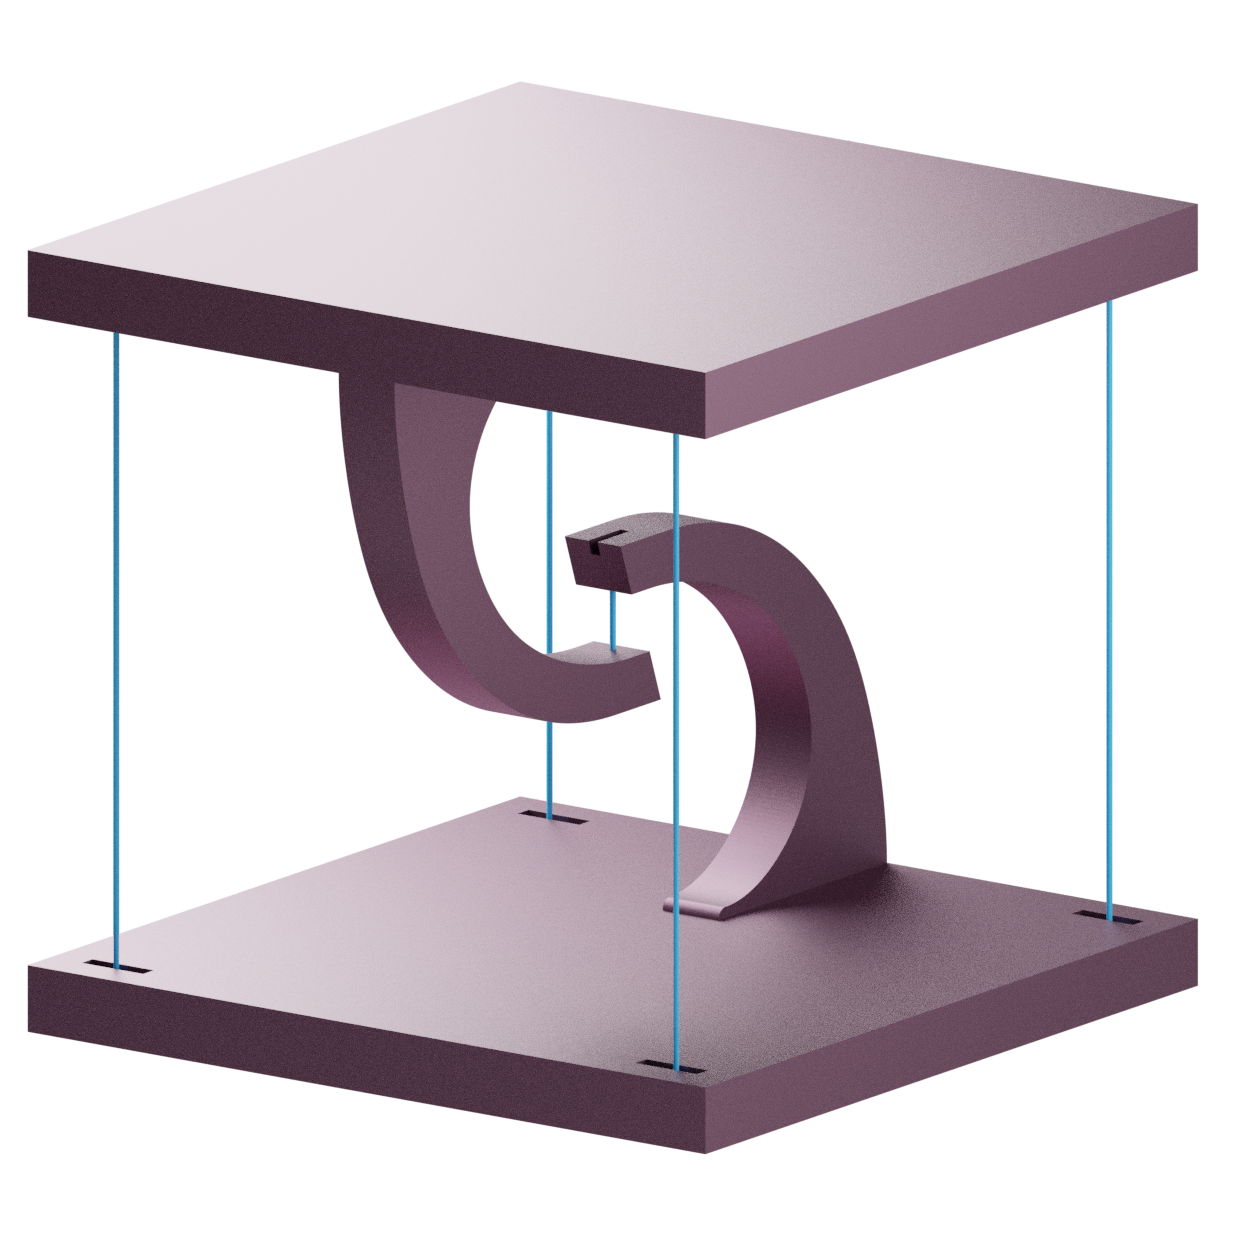
\includegraphics[width=8cm]{tensegrity.png}
    \caption{Tensegrity structure}
    \label{tensegrity}
\end{figure}
The tensegrity structure is held by compression and a network of compression to create the illusion of a floating platform. The structure is made such that it cannot be toppled over so that it always appears to be floating. This was designed in this way to attract casual passers-by whose interest may be piqued by the ``floating'' structure.

\begin{figure}[H]
    \centering
    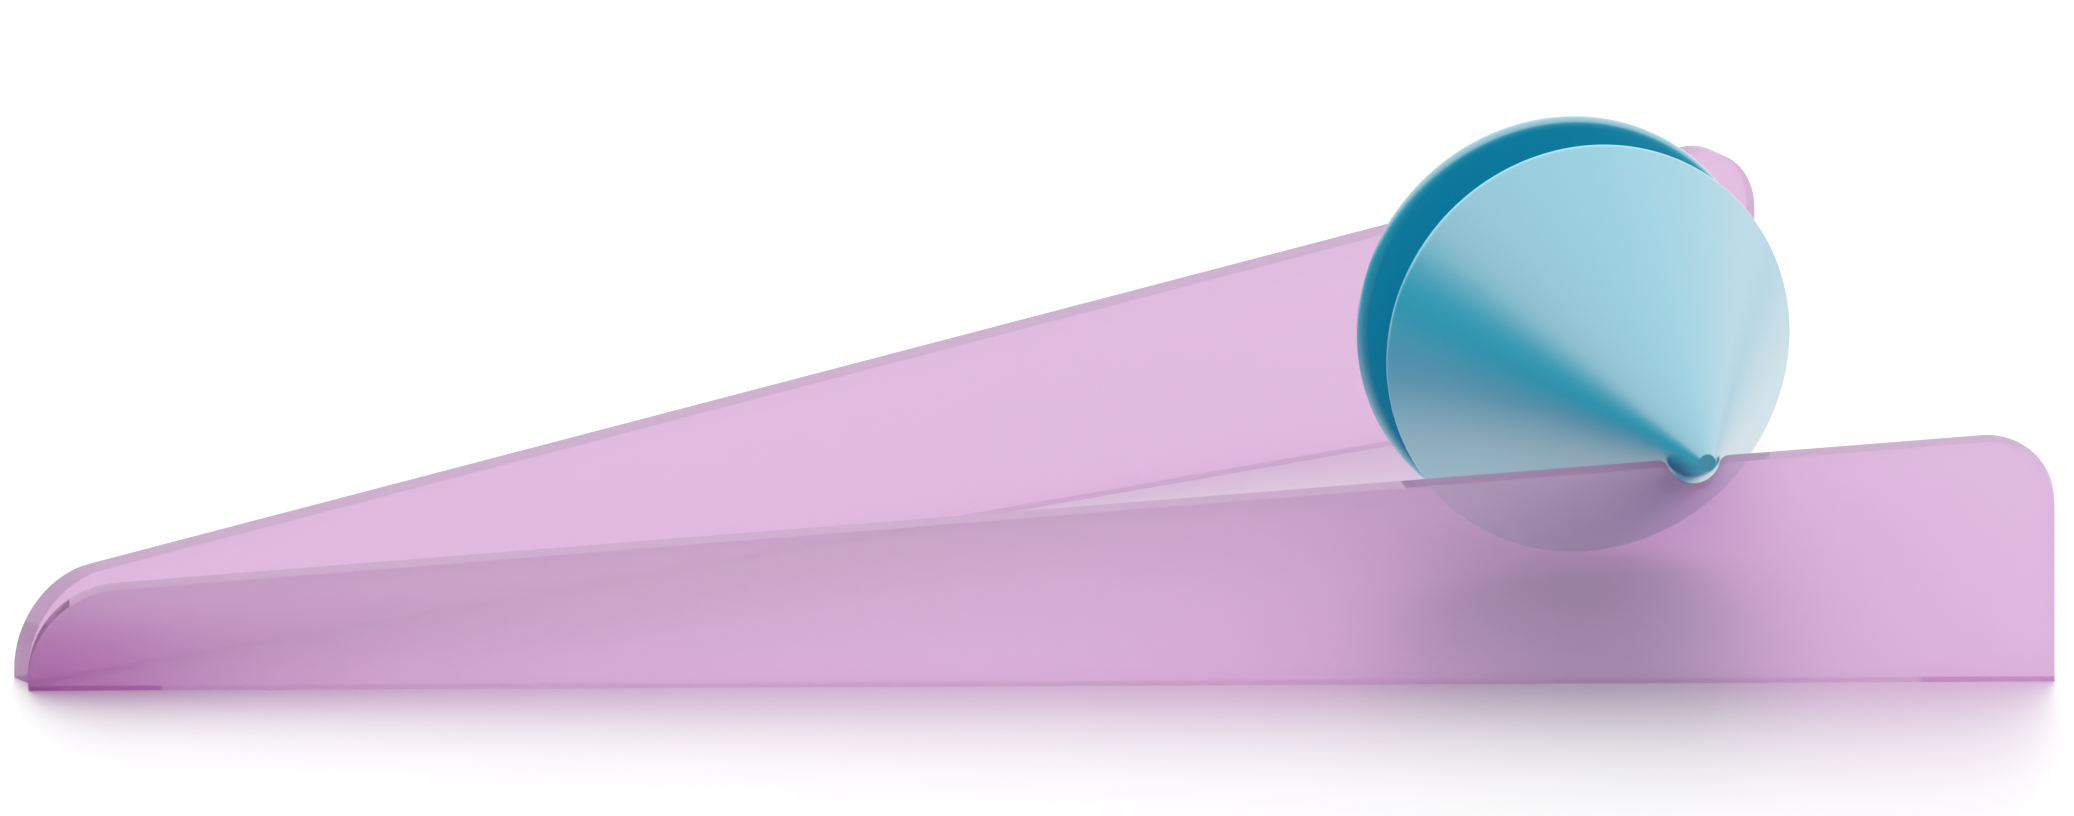
\includegraphics[width=8cm]{holder-pink-darker-FFFFFF.png}
    \caption{Uphill roller}
    \label{}
\end{figure}
The uphill roller is an illusionary demonstration that showcases the importance of centre of gravity. A double cone rolls down 2 rails, the distance between which is increasing. The angles of the spreading rails, double cone and slope of the rails are chosen carefully such that when the cone rolls down the spreading rails, it appears to be rolling up the slope. Figure~\ref{sticker} shows the information graphic that will accompany the model, with a QR code that brings the attendee to a website for an explanation of the mechanics behind the model.
\begin{figure}[H]
    \centering
    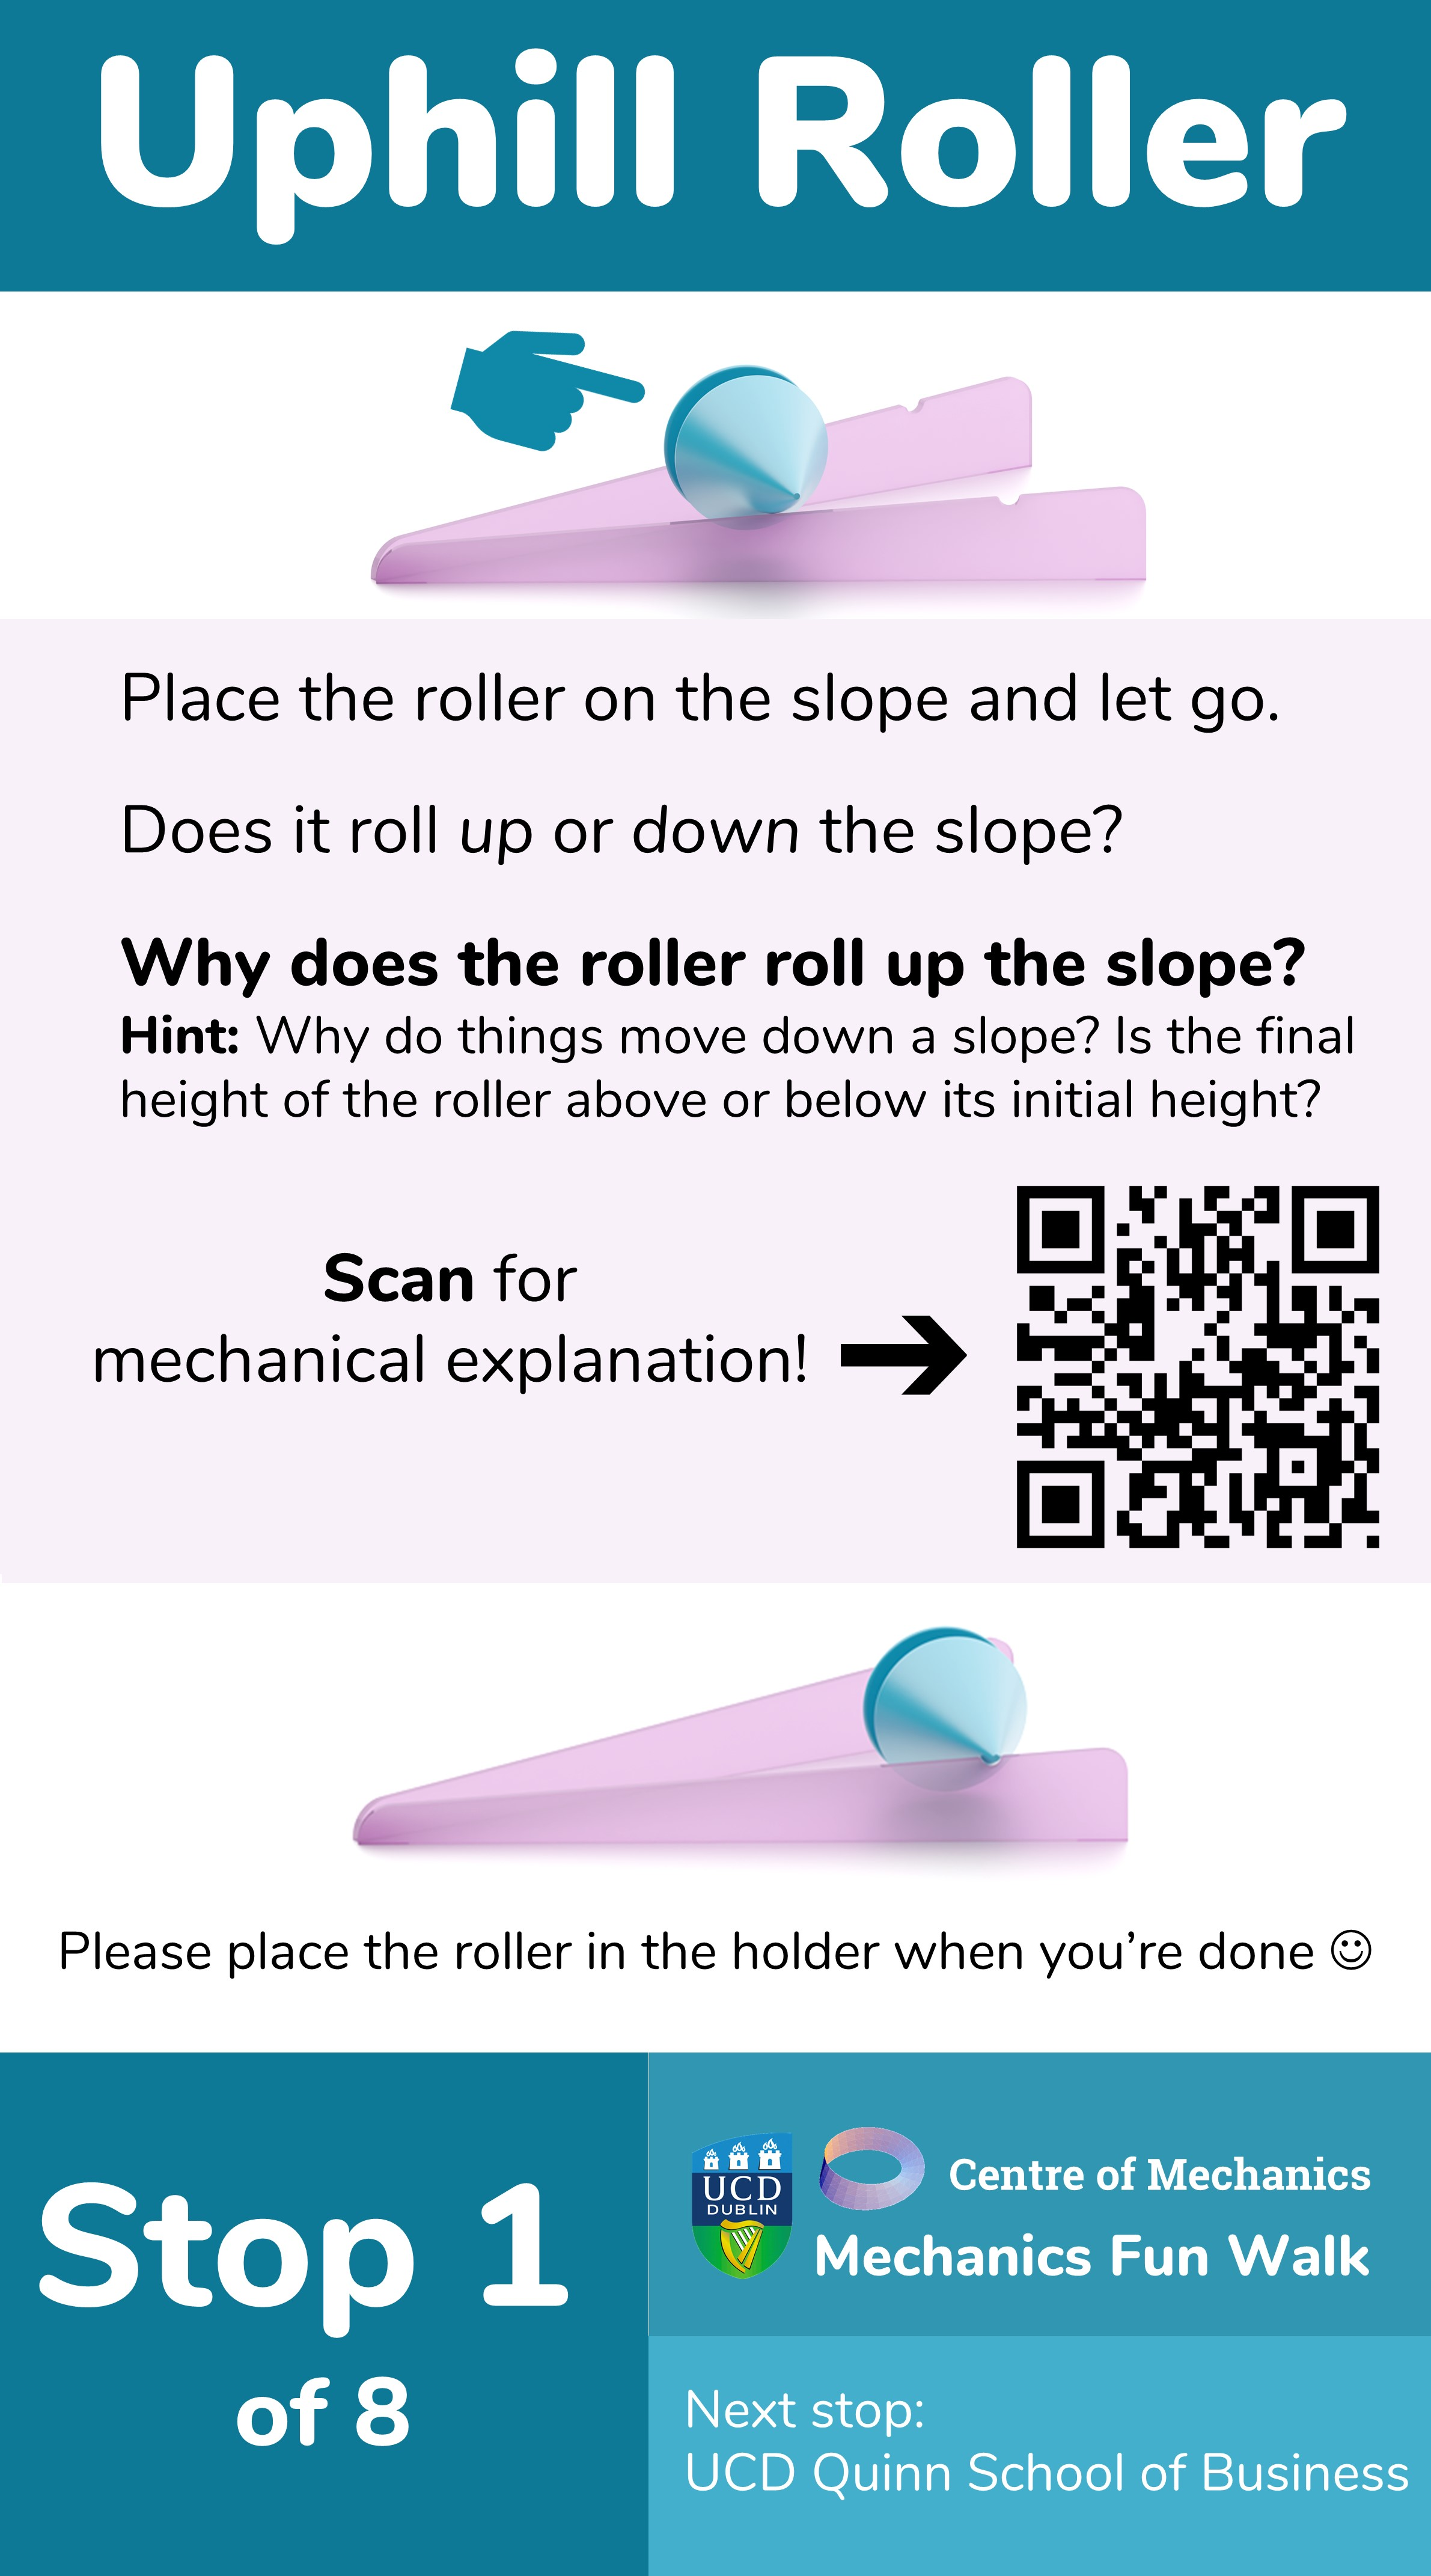
\includegraphics[width=6.5cm]{uphillrollersticker.jpg}
    \caption{Information graphic for uphill roller demonstration}
    \label{sticker}
\end{figure}

\section{Project Plan}
The brachistochrone and Galton board models will be used to showcase this project to attract investment and funding for the project. 
% something about permission from UCD?

When the funding has been attained, the other models will be created and distributed across the campus in University College Dublin. A webpage will be set up for the QR codes to link to.






\newpage

\bibliography{MechanicsWalk}

\end{document}
